% !TEX root = ../../semexp-thesis.tex

\section{Semantic Completions}
\label{sec:implementation/completions}

Our implementation of semantic completions reuses the framework of the suggestion space for tracking the experiments of programmers.

\begin{figure}
	\centering
	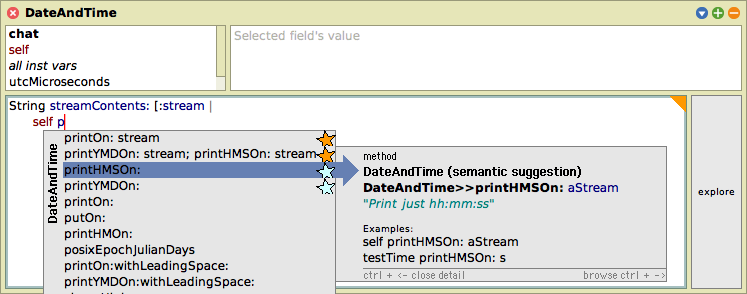
\includegraphics[width=\textwidth]{02_completions/screenshot.png} % TODO screenshot: [COULD?] improve resolution, maybe grow left pane slightly and shrink right pane/inspector slightly
	\caption[Our integration of semantic completions into the \name{Autocompletion} tool for Squeak.]{
		Our integration of semantic completions into the \name{Autocompletion} tool for Squeak, here invoked frmo an inspector on a \code{DateAndTime} object.
		Correlated names are displayed with a \bold{\textcolor[HTML]{598db3}{blue}} star and generated expressions are displayed with an \bold{\textcolor{orange!80!black}{orange}} star.
		Programmers can select an entry to read details such as documentation, usage examples, or a preview of its result, and press Tab to insert it into their editor.
	}
	\label{fig:implementation/completions}
\end{figure}

For the user interface of completions, we use the \name{Autocompletion} package\footnote{\url{https://github.com/LeonMatthes/Autocompletion}} and employ its \code{ECEntryHook} interface~(\cref{fig:implementation/completions}).
We contribute two new types of completion entries: \emph{correlated names} and \emph{generated expressions}.

First, we provide regular selectors and variable names based on correlated suggestion artifacts from the suggestion space and merge them with traditional \name{Autocompletion} entries.
This considers the original ranking of entries, which is only based on alphabetical order and most recently used date, and enhances it with their semantic relevance.
We hook into the presentation of entries to enrich suggested names with usage information mined from their preceding similar code artifacts as well as related documentation.

Second, we include contextualized generated expressions~(see \cref{sec:suggestions/generation}) into the completion menu.
Analogously to the suggestion space, semantic completions are computed asynchronously in the background to avoid noticable delays in the user interface.

To generate a preview of the result of generated expressions, we run them in the editor context inside an isolated sandbox of \name{SimulationStudio} and include the results in the presentation of each entry.
